% \subsection{Relaciones constitutivas}

% En el caso de un sólido tridimensional isotrópico la relación esfuerzo-deformación está dada por la Ley de Hooke, 
% expresada en términos matemáticos como:

% \begin{equation}\label{eq:ecdef}
% \vec{\varepsilon} = 
% \left\{\begin{matrix}
% \varepsilon_{xx} \\ \varepsilon_{yy} \\ \varepsilon_{zz} \\ \varepsilon_{xy} \\ \varepsilon_{yz} \\ \varepsilon_{zx}
% \end{matrix}\right\} = 
% \left[ C \right] \vec{\sigma} + \vec{\varepsilon_0} = 
% \left[ C \right]
% \left\{\begin{matrix}
% \sigma_{xx} \\ \sigma_{yy} \\ \sigma_{zz} \\ \sigma_{xy} \\ \sigma_{yz} \\ \sigma_{zx}
% \end{matrix}\right\} + 
% \left\{\begin{matrix}
% \varepsilon_{xx}_0 \\ \varepsilon_{yy}_0 \\ \varepsilon_{zz}_0 \\ \varepsilon_{xy}_0 \\ \varepsilon_{yz}_0 \\ \varepsilon_{zx}_0
% \end{matrix}\right\}
% \end{equation}

% Donde $[C]$ es la matriz de constantes elásticas definida por:

% \begin{equation}
% [C] = \frac{1}{E}
% \left[\begin{matrix}
% 1 & -\nu & -\nu & 0 & 0 & 0 \\
% -\nu & 1 & -\nu & 0 & 0 & 0 \\
% -\nu & -\nu & 1 & 0 & 0 & 0 \\
% 0 & 0 & 0 & 2(1+\nu) & 0 & 0 \\
% 0 & 0 & 0 & 0 & 2(1+\nu) & 0 \\
% 0 & 0 & 0 & 0 & 0 & 2(1+\nu) \\
% \end{matrix}\right]
% \end{equation}

% $\vec{\varepsilon_0}$ es el vector de esfuerzos iniciales, $E$ es el módulo de Young y $\nu$ el coeficiente de Poisson del 
% material.\\

% Algunas veces la expresión de esfuerzos en términos de deformaciones puede ser necesaria. Incluyendo las deformaciones 
% térmicas, la ecuación \ref{eq:ecdef} puede ser invertida para obtener:

% \begin{equation}
% \vec{\sigma} = 
% \left\{\begin{matrix}
% \sigma_{xx} \\ \sigma_{yy} \\ \sigma_{zz} \\ \sigma_{xy} \\ \sigma_{yz} \\ \sigma_{zx}
% \end{matrix}\right\} = 
% \left[ D \right] (\vec{\varepsilon} - \vec{\varepsilon_0})= 
% \left[ D \right] 
% \left\{\begin{matrix}
% \varepsilon_{xx} \\ \varepsilon_{yy} \\ \varepsilon_{zz} \\ \varepsilon_{xy} \\ \varepsilon_{yz} \\ \varepsilon_{zx}
% \end{matrix}\right\} - 
% \frac{E\alpha T}{1-2\nu}
% \left\{\begin{matrix}
% 1 \\ 1 \\ 1 \\ 0 \\ 0 \\ 0
% \end{matrix}\right\} 
% \end{equation}

% Donde la matriz $[D]$ está dada por:

% \begin{equation}
% [C] = \frac{E}{(1+\nu)(1-2\nu)}
% \left[\begin{matrix}
% 1-\nu & \nu & \nu & 0 & 0 & 0 \\
% \nu & 1-\nu & \nu & 0 & 0 & 0 \\
% \nu & \nu & 1-\nu & 0 & 0 & 0 \\
% 0 & 0 & 0 & \frac{1-2\nu}{2} & 0 & 0 \\
% 0 & 0 & 0 & 0 & \frac{1-2\nu}{2} & 0 \\
% 0 & 0 & 0 & 0 & 0 & \frac{1-2\nu}{2} \\
% \end{matrix}\right]
% \end{equation}

% En el caso de problemas bidimensionales, dos tipos de distribuciones de esfuerzos son posibles: esfuerzo plano 
% y deformación plana.

% \subsubsection{Esfuerzo plano}

% La consideración de esfuerzo plano es aplicable para cuerpos en los cuales su dimensión en una dirección es muy 
% pequeña comparada con las otras. En el caso de esfuerzo plano se asume que:

% \begin{equation}
% \sigma_{zz} = \sigma_{zx} = \sigma_{yz} = 0
% \end{equation}

% Donde $z$ representa la dirección perpendicular al plano de la placa mostrada en la figura \ref{fig:fg1}, 
% y los componentes de esfuerzo no varían a través del espesor de la placa.

% \begin{center}
% 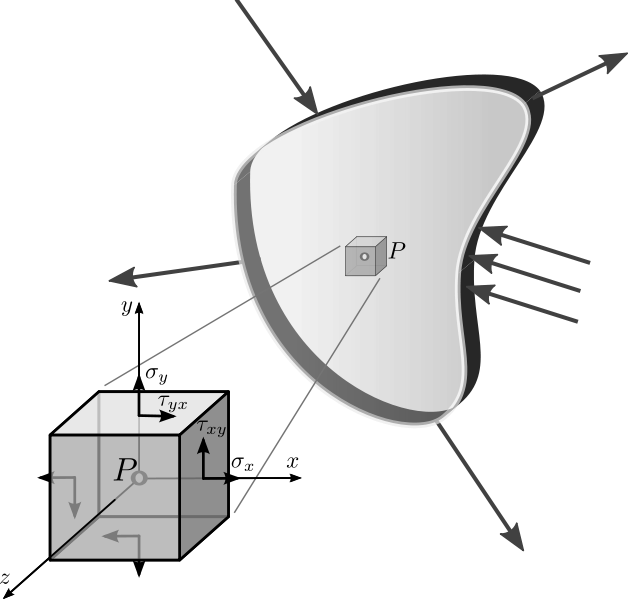
\includegraphics[scale=0.35]{src/ch2/plane_stress.png}
% \captionof{figure}{Esfuerzo plano}
% \label{fig:fg1}
% \end{center}

% Entonces, las relaciones esfuerzo deformación se reducen a:

% \begin{equation}
% \vec{\varepsilon} = [C] \vec{\sigma} + \vec{\varepsilon_0}
% \end{equation}

% donde:

% \begin{equation}
% \vec{\varepsilon} = 
% \left\{\begin{matrix}
% \varepsilon_{xx} \\ \varepsilon_{yy} \\ \varepsilon_{xy}
% \end{matrix}\right\}
% \end{equation}

% \begin{equation}
% \vec{\sigma} = 
% \left\{\begin{matrix}
% \sigma_{xx} \\ \sigma_{yy} \\ \sigma_{xy}
% \end{matrix}\right\}
% \end{equation}

% \begin{equation}
% [C] = \frac{1}{E}
% \left[\begin{matrix}
% 1 & -\nu & 0 \\
% -\nu & 1 & 0 \\
% 0 & 0 & 2(1+\nu) \\
% \end{matrix}\right]
% \end{equation}

% \begin{equation}
% \vec{\varepsilon_0} = 
% \left\{\begin{matrix}
% \varepsilon_{xx_0} \\ \varepsilon_{yy_0} \\ \varepsilon_{xy_0}
% \end{matrix}\right\} =
% \alpha T 
% \left\{\begin{matrix}
% 1 \\ 1 \\ 0 \\
% \end{matrix}\right\}
% \end{equation}

% En el caso de deformaciones térmicas,

% \begin{equation}
% \vec{\sigma} = [D] (\vec{\varepsilon} - \vec{\varepsilon_0}) = 
% [D] \vec{\varepsilon} - 
% \frac{E\alpha T}{1-\nu} 
% \left\{\begin{matrix}
% 1 \\ 1 \\ 0 \\
% \end{matrix}\right\}
% \end{equation}

% Con, 

% \begin{equation}
% [D] = \frac{E}{1-\nu^2}
% \left[\begin{matrix}
% 1 & \nu & 0 \\
% \nu & 1 & 0 \\
% 0 & 0 & \frac{1-\nu}{2} \\
% \end{matrix}\right]
% \end{equation}

% En el caso de esfuerzo plano la componente de la deformación en el plano $z$, será diferente de cero, debido al 
% efecto del coeficiente de Poisson, estando dada  por la expresión:

% \begin{equation}
% \varepsilon_{zz} = -\frac{\nu}{E} (\sigma_{xx} + \sigma_{yy}) + \alpha T = 
% \frac{-\nu}{1-\nu} (\varepsilon_{xx} + \varepsilon_{yy}) +  
% \frac{1+\nu}{1-\nu} \alpha T
% \end{equation}

% Mientras que, 

% \begin{equation}
% \varepsilon_{yz} = \varepsilon_{zx} = 0
% \end{equation}


% \subsubsection{Deformación plana}

% La consideración de deformación plana es aplicable para sólidos largos y cuya geometría y cargas no varían de 
% manera significativa en la dirección longitudinal.\\

% En este caso las ecuaciones de esfuerzo-deformación tridimensional se reducen a:

% \begin{equation}
% \vec{\varepsilon} = [C] \vec{\sigma} + \vec{\varepsilon_0}
% \end{equation}

% donde:

% \begin{equation}
% \vec{\varepsilon} = 
% \left\{\begin{matrix}
% \varepsilon_{xx} \\ \varepsilon_{yy} \\ \varepsilon_{xy}
% \end{matrix}\right\}
% \end{equation}

% \begin{equation}
% \vec{\sigma} = 
% \left\{\begin{matrix}
% \sigma_{xx} \\ \sigma_{yy} \\ \sigma_{xy}
% \end{matrix}\right\}
% \end{equation}

% \begin{equation}
% [C] = \frac{1+\nu}{E}
% \left[\begin{matrix}
% 1-\nu & -\nu & 0 \\
% -\nu & 1-\nu & 0 \\
% 0 & 0 & 2 \\
% \end{matrix}\right]
% \end{equation}

% \begin{equation}
% \vec{\varepsilon_0} = 
% \left\{\begin{matrix}
% \varepsilon_{xx_0} \\ \varepsilon_{yy_0} \\ \varepsilon_{xy_0}
% \end{matrix}\right\} =
% (1+\nu) \alpha T 
% \left\{\begin{matrix}
% 1 \\ 1 \\ 0 \\
% \end{matrix}\right\}
% \end{equation}

% En el caso de deformaciones térmicas,

% \begin{equation}
% \vec{\sigma} = [D] (\vec{\varepsilon} - \vec{\varepsilon_0}) = 
% [D] \vec{\varepsilon} - 
% \frac{E\alpha T}{1-2\nu} 
% \left\{\begin{matrix}
% 1 \\ 1 \\ 0 \\
% \end{matrix}\right\}
% \end{equation}

% Con, 

% \begin{equation}
% [D] = \frac{E}{(1+\nu)(1-2\nu)}
% \left[\begin{matrix}
% 1-\nu & \nu & 0 \\
% \nu & 1-\nu & 0 \\
% 0 & 0 & \frac{1-2\nu}{2} \\
% \end{matrix}\right]
% \end{equation}

% \begin{center}
% 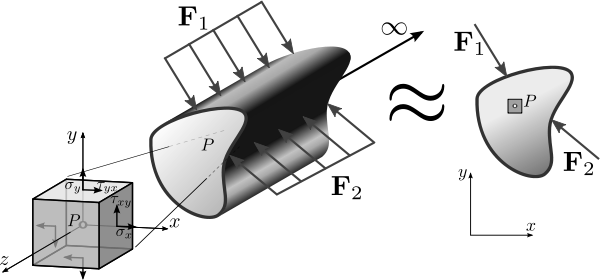
\includegraphics[scale=0.55]{src/ch2/plane_strain.png}
% \captionof{figure}{Deformación plana}
% \label{fig:fg2}
% \end{center}

% El componente de esfuerzo en la dirección $z$ no será nulo debido a los efectos del coeficiente de Poisson, y está 
% dado por:

% \begin{equation}
% \sigma_{zz} = \nu(\sigma_{xx}+\sigma_{yy}) - E \alpha T
% \end{equation}

% y, 

% \begin{equation}
% \sigma_{yz} = \sigma_{zx} = 0
% \end{equation}

% \subsection{Relaciones deformación-desplazamiento}

% La forma deformada de un cuerpo elástico bajo una determinada configuración de cargas y distribución de temperaturas 
% pueden ser descritas completamente por tres componentes de desplazamiento $u, v$ y $w$ paralelas a las direcciones 
% $x, y$ y $z$ respectivamente. En general, cada una de estas componentes $u,v$ y $w$ es una función de las 
% coordenadas $x,y$ y $z$. Las deformaciones inducidas en el sólido pueden ser expresadas en términos de los 
% desplazamientos $u,v$ y $w$.\\

% Si los desplazamientos se consideran muy pequeños, la deformaciones pueden ser expresadas como:

% \begin{subequations}
% \begin{eqnarray}
% \varepsilon_{xx} = \frac{du}{dx} \\
% \varepsilon_{yy} = \frac{dv}{dy} \\
% \varepsilon_{zz} = \frac{dw}{dz} \\
% \varepsilon_{xy} = \frac{du}{dy} + \frac{dv}{dx} \\
% \varepsilon_{yz} = \frac{dw}{dy} + \frac{dv}{dz} \\
% \varepsilon_{zx} = \frac{du}{dz} + \frac{dw}{dx} \\
% \end{eqnarray}
% \end{subequations}


% \subsection{Ecuaciones de equilibrio}

% \subsubsection{Equilibrio externo}

% Si un sólido está en equilibrio bajo ciertas condiciones de carga, las fuerzas reactivas y momentos desarrollados en 
% los puntos de soporte deben balancear las fuerzas y momentos externos aplicados. Haciendo referencia a la figura 
% \ref{fig:externalforces}, sean $\phi_x, \phi_y, \phi_z$ las fuerzas de cuerpo, $\Phi_x, \Phi_y, \Phi_z$ las 
% fuerzas de superficie, $P_x, P_y, P_z$ las fuerzas concentradas externas, y $Q_x, Q_y, Q_z$ los momentos externos 
% aplicados. Entonces, las ecuaciones de equilibrio externo pueden establecerse como:

% \begin{eqnarray}
% \int_S \Phi_x ds + \int_V \phi_x dV + \sum P_x = 0 \nonumber \\
% \int_S \Phi_y ds + \int_V \phi_y dV + \sum P_y = 0 \\
% \int_S \Phi_z ds + \int_V \phi_z dV + \sum P_z = 0 \nonumber
% \end{eqnarray}

% \begin{center}
% 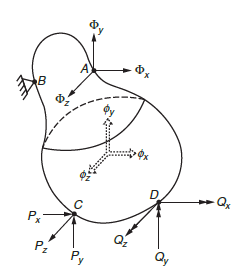
\includegraphics[scale]{src/ch2/equillibrium_force.png}
% \captionof{figure}{Fuerzas de equilibrio externo}
% \label{fig:externalforces}
% \end{center}

% Para el equilibrio de momentos:

% \begin{eqnarray}
% \int_S (\Phi_zy - \Phi_{y}z) ds + \int_V (\phi_zy - \phi_{y}z) dV + \sum Q_x = 0 \nonumber \\
% \int_S (\Phi_x z - \Phi_z x) ds + \int_V (\phi_x z - \phi_z x) dV + \sum Q_y = 0 \\
% \int_S (\Phi_{y}x - \Phi_x y) ds + \int_V (\phi_{y}x - \phi_x y) dV + \sum Q_z = 0 \nonumber
% \end{eqnarray}

% Donde $S$ es la superficie y $V$ el volumen del cuerpo sólido.


% \subsubsection{Equilibrio interno}

% Debido a las aplicación de cargas, se desarrollan esfuerzos dentro del sólido. Si consideramos 
% un elemento de material dentro del sólido, este debería estar en equilibrio debido a esos 
% esfuerzos internos desarrollados.\\

% Teoricamente, el estado de esfuerzos en cualquier punto de un cuerpo cargado está completamente definido 
% en términos de nueve componentes de esfuerzo: $\sigma_{xx}, \sigma_{yy}, \sigma_{zz}, \sigma_{xy}, \sigma_{yx}, 
% \sigma_{yz}, \sigma_{zy}, \sigma_{zx}, \sigma_{xz} $, donde los primeros tres son las componentes normales y los restantes 
% son esfuerzos cortantes. Las ecuaciones de equilibrio interno relativas a los nueve componentes de esfuerzo pueden ser 
% obtenidas considerando el equilibrio de momentos y fuerzas actuando en el volumen elemental mostrado en 
% la figura \ref{fig:internalforces}. El equilibrio de momentos alrededor de los ejes $x,y,z$, asumiendo que no existen 
% momentos en el sólido, derivan en las siguientes relaciones:

% \begin{equation}
% \sigma_{yx} = \sigma_{xy}, \,\,\,\, \sigma_{zy} = \sigma_{yz}, \,\,\,\, \sigma_{xz} = \sigma_{zx}
% \end{equation}

% \begin{center}
% 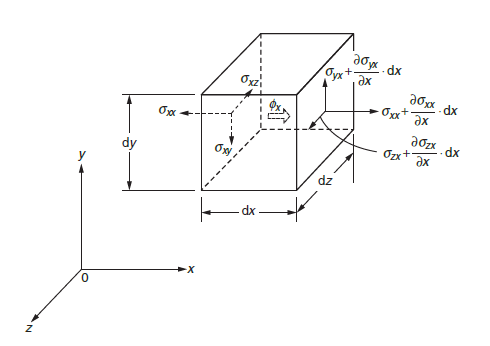
\includegraphics[scale]{src/ch2/internal_force.png}
% \captionof{figure}{Fuerzas de equilibrio interno}
% \label{fig:internalforces}
% \end{center}

% Estas ecuaciones muestran que el estado de esfuerzos en cualquier punto puede ser completamente definido por 
% los seis componentes $\sigma_{xx}, \sigma_{yy}, \sigma_{zz}, \sigma_{xy}, \sigma_{yz}, \sigma_{zx} $. 
% El equilibrio de fuerzas en las direcciones $x,y,z$ proporcionan las siguientes ecuaciones diferenciales de 
% equilibrio:

% \begin{eqnarray}
% \frac{\partial \sigma_{xx}}{\partial x} + \frac{\partial \sigma_{xy}}{\partial y} + 
% \frac{\partial \sigma_{zx}}{\partial z} + \phi_{x} = 0 \nonumber \\
% \frac{\partial \sigma_{xy}}{\partial x} + \frac{\partial \sigma_{yy}}{\partial y} + 
% \frac{\partial \sigma_{yz}}{\partial z} + \phi_{y} = 0 \\
% \frac{\partial \sigma_{zx}}{\partial x} + \frac{\partial \sigma_{yz}}{\partial y} + 
% \frac{\partial \sigma_{zz}}{\partial z} + \phi_{z} = 0 \nonumber
% \end{eqnarray}

% donde $\phi_x, \phi_y$ y $\phi_z$, son las fuerzas de cuerpo por unidad de volumen actuando a lo largo 
% de las direcciones $x,y$ y $z$, respectivamente.\\

% Para un problema bidimensional, existen solamente tres componentes de esfuerzo independientes, 
% $(\sigma_{xx},\sigma_{yy},\sigma_{xy})$ y las ecuaciones de equilibrio se reducen a:

% \begin{eqnarray}
% \frac{\partial \sigma_{xx}}{\partial x} + \frac{\partial \sigma_{xy}}{\partial y} + \phi_x = 0 \nonumber \\
% \frac{\partial \sigma_{xy}}{\partial x} + \frac{\partial \sigma_{yy}}{\partial y} + \phi_y = 0 
% \end{eqnarray}

% En problemas unidimensionales, sólo estará presente un componente de esfuerzo: $\sigma_{xx}$. Entonces, 
% las ecuaciones de equilibrio se reducen a:

% \begin{equation}
% \frac{\partial \sigma_{xx}}{\partial x} + \phi_x = 0
% \end{equation}






% \section{Teoría de contactos}

% \subsection{Introducción}

% Considere el movimiento dependiente del tiempo de dos cuerpos ocupando las regiones $B^1$ y $B^2$ 
% en su configuración deformada en el tiempo cero. Asuma que la intersección

% $$
% B^1 \cap B^2 = \emptyset
% $$

% es satisfecha. Sean $\partial B^1$ y $\partial B^1$ quienes denotan las fronteras de $B^1$ y $B^2$ 
% respectivamente. En un tiempo posterior, estos cuerpos ocupan las regiones $b^1$ y $b^2$ delimitadas 
% por $\partial b^1$ y $\partial b^2$ como se muestra en la figura \ref{fig:refanddef}. Debido a que la 
% configuración deformada no puede penetrar:

% $$
% \left( b^1 - \partial b^1 \right) \cap b^2 = \emptyset
% $$

% Mientras $\left( \partial b^1 \cap \partial b^2 \right) = \emptyset$, las ecuaciones de movimiento 
% permanecen desacopladas. En las anteriores y siguientes ecuaciones, el superíndice derecho $\alpha$ 
% $(=1,2)$ denota el cuerpo al cual la cantidad hace referencia.

% \begin{center}
% 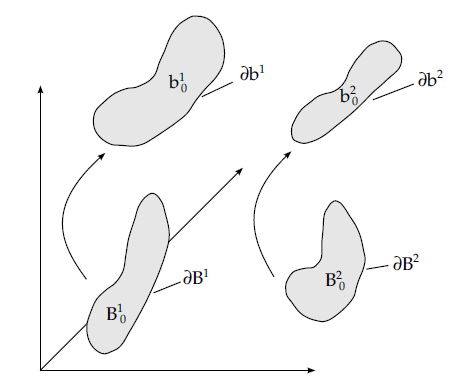
\includegraphics[scale=0.6]{src/ch2/ref_and_def.png}
% \captionof{figure}{Configuración de referencia y deformada}
% \label{fig:refanddef}
% \end{center}

% Antes de dar una descripción detallada de la teoría de contactos, algunos cuestiones adicionales 
% referentes a la terminología deben ser agregadas. Las superficies $\partial b^1$ y $\partial b^2$ 
% de los cuerpos discretizados $b^1$ y $b^2$ vienen a ser las superficies \textit{maestra} 
% y \textit{esclava}, respectivamente. La selección de las superficies maestra y esclava es 
% arbitraria cuando el tratamiento simétrico de penalización es utilizado. De lo contrario, 
% la superficie de malla más \textit{burda} debe ser elegida como maestra a menos que 
% exista una gran diferencia en las densidades de masa, en cuyo caso se recomienda definir 
% como superficie maestra al del material con mayor densidad de masa. Los puntos nodales 
% que definen $\partial b^1$ son llamados nodos maestros y los nodos que definen $\partial b^2$ 
% son llamados nodos esclavos. Cuando $\left( \partial b^1 \cap \partial b^2 \right) \neq \emptyset$, 
% las restricciones son impuestas para prevenir la penetración. Los superíndices derechos se 
% utilizan cuando una variable se refiere tanto a la superficie maestra $\partial b^1$ o 
% a la sueperficie esclava $\partial b^2$, consecuentemente estos superíndices se descartan 
% en el desarrollo siguiente.

% \subsection{\textit{Slave search}}

% Esta búsqueda encuentra para cada nodo esclavo su punto más cercano en la superficie maestra. 
% Las líneas dibujadas de un nodo esclavo a sus puntos más cercanos serán perpendiculares a la 
% superficie maestra, a menos que el punto se encuentre en la intersección de dos segmentos 
% maestros, donde un segmento está definido a ser un elemento de superficie de 3 o 4 nodos.\\

% Considere un nodo esclavo, $n_s$, deslizándose en una superficie maestra suave a tramos y 
% asuma que una búsqueda de la superficie maestra ha encontrado el nodo maestro, $m_s$, 
% situado cerca de $n_s$. La figura \ref{fig:slave_search} representa una porción 
% de una superficie maestra con nodos referenciados como $m_s$ y $n_s$. Si $m_s$ 
% y $n_s$ no coinciden, para $n_s$ por lo general se puede demostrar que se encuentra 
% en un segmento $s_1$  mediante el siguiente test:

% \begin{equation}
% (\mathbf{c_i} x \mathbf{s}) \cdot (\mathbf{c_i} x \mathbf{c_{i+1}}) > 0
% \end{equation}

% \begin{equation}
% (\mathbf{c_i} x \mathbf{s}) \cdot (\mathbf{s} x \mathbf{c_{i+1}}) > 0
% \end{equation}

% donde el vector $\mathbf{c_i}$ y $\mathbf{c_{i+1}}$

% \begin{center}
% 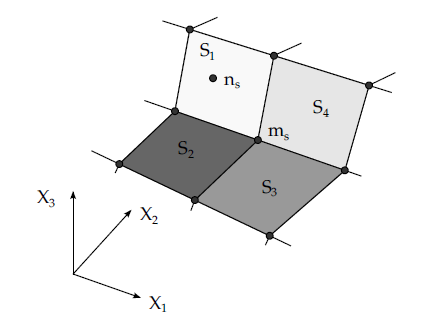
\includegraphics[scale=0.6]{src/ch2/slave_search.png}
% \captionof{figure}{Slave search}
% \label{fig:slave_search}
% \end{center}


% \subsection{Algoritmo de contacto superficie-superficie}

% Este implica un enfoque simétrico de dos pasos con un parámetro 
% de partición, $\beta$, que se establece entre la unidad positiva y negativa, donde $\beta=1$ 
% y $\beta=-1$ corresponden a tratamiento de una forma con la superficie \textit{maestra} 
% acumulando masa y fuerzas de la superficie \textit{esclava} (para $\beta = 1$) y viceversa 
% (para $\beta = -1$). ~\cite{lsdyna-manual} \\ 

% En este enfoque de restricción las aceleraciones, velocidades y desplazamientos se actualizan 
% primero a una configuración de prueba sin tener en cuenta las interacciones. Después de la 
% actualización, una fuerza de penetración es calculada para el nodo esclavo como una función 
% de la distancia de penetración $\Delta L$:

% $$
% \mathbf{\f_p} = \frac{m_s \Delta L}{\Delta t^2}\mathbf{n},
% $$

% Donde $\mathbf{n}$ es el vector normal a la superficie maestra.\\

% Se desea que la respuesta de la componente normal del vector de aceleración del nodo esclavo, 
% $\mathbf{a_s}$, de un nodo esclavo residiendo en un segmento maestro $k$ sea consistente con 
% el movimiento del segmento maestro en su porción de contacto $(s_c,t_c)$, por ejemplo:

% $$
% a_s = \phi_1 (s_c,t_c) a_{nk}^1 + \phi_2 (s_c,t_c) a_{nk}^2 + \phi_3 (s_c,t_c) a_{nk}^3 + \phi_4 (s_c,t_c) a_{nk}^4
% $$

% Para cada nodo esclavo en contacto y penetrando a través de la superficie maestra en 
% su configuración de prueba, su masa nodal y fuerza de penetración dadas por la ecuación 
% [REVISAR (Poner aquí referencia)] es acumulada a una masa y vector de fuerza global de 
% la superficie maestra.

% $$
% \left(
% m_k + \sum_s m_{ks}
% \right)
% \mathbf{a_{nk}}
% =
% \sum_s \mathbf{f_{ks}}
% $$

% donde:

% $$
% m_{ks} = \phi_k m_s
% $$

% $$
% \mathbf{f_{ks}} = \phi{k} \mathbf{f_s}
% $$

% Después de resolver la ecuación [REVISAR] para el vector de aceleración, $\mathbf{a_{nk}}$, podemos 
% obtener la corrección de aceleración para el nodo esclavo como:

% $$
% \mathbf{a_{ns}} = \mathbf{a_s} - \frac{f_p}{m_s}
% $$

% El proceso anterior es repetido después de invertir las definiciones de \textit{maestro-esclavo}. 
% En el paso final la corrección final promediada al vector de aceleración es encontrada:

% $$
% \mathbf{a_n^{final}} = \frac{1}{2} (1-\beta) \mathbf{a_n^{1st pass}} + 
% \frac{1}{2} (1-\beta) \mathbf{a_n^{2nd pass}} 
% $$

% Y se usa para calcular la aceleración final en el tiempo $n+1$

% $$
% \mathbf{a}^{n+1} = \mathbf{a}^{prueba} + \mathbf{a}_n^{final}
% $$

% La fricción resiste la velocidad tangencial relativa del nodo esclavo con respecto a 
% la superficie maestra. Esta velocidad relativa se expresa como:

% $$
% \mathbf{v_r} = \mathbf{v_s} - 
% \left(
% \phi_1 \mathbf{v}_k^1 + \phi_2 \mathbf{v}_k^2 + \phi_3 \mathbf{v}_k^3 + \phi_4 \mathbf{v}_k^4
% \right)
% $$

% la componente normal de la velocidad al segmento maestro:

% $$
% \mathbf{v_t} = \mathbf{v_r} - (\mathbf{n} \cdot \mathbf{v_r}) \mathbf{n}
% $$

% Una fuerza tangencial de prueba es calculada que cancelará la velocidad tangencial:

% $$
% \mathbf{f^{\ast}} = \frac{m_s v_t}{\Delta t}
% $$

% Donde $v_t$ es la magnitud del vector de velocidad tangencial.

% $$
% v_t = \sqrt{\mathbf{v}_t \cdot \mathbf{v}_t}
% $$

% La magnitud de la fuerza tangencial es limitada por la magnitud del producto de la constante de fricción 
% de Coulomb con la fuerza normal definido como:

% $$
% f_n = m_s \mathbf{a}_{ns} \cdot \mathbf{n}
% $$

% La fuerza limitada es, por lo tanto:

% $$
% F_y = m |\mathbf{f}_n|
% $$

% y 

% $$
% \mathbf{f}^{n+1} = \mathbf{f^{\ast}} \,\,\, if \,\,\, |\mathbf{f^{\ast}}| = F_y
% $$

% $$
% \mathbf{f}^{n+1} = \frac{F_y \mathbf{f^{\ast}}}{|\mathbf{f^{\ast}}|} \,\,\, if \,\,\, |\mathbf{f^{\ast}}| > F_y
% $$

% Por lo tanto, usando las ecuaciones anteriores la modificiación a la componente de  aceleración tangencial 
% del nodo esclavo está dado por:

% $$
% \mathbf{a_t} = \min\left( \mu \mathbf{a_{nt}} \cdot \mathbf{n} , \frac{|\mathbf{v_s}|}{\Delta t} \right)
% $$

% el cual debe actuar en la dirección del vector tangencial definido como:

% $$
% \mathbf{n_t} = \frac{\mathbf{v_t}}{v_t}
% $$

% Las correcciones a las componentes de aceleración del nodo esclavo y maestro son: 

% $$
% a_{ts} = a_{t} \mathbf{n_t}
% $$

% $$
% \mathbf{a_{tk}} = - \phi_k \frac{a_s m_s}{m_k} \mathbf{n_t}
% $$

% El proceso anterior se repite después de invertir la definición de esclavo y maestro. En el 
% paso final la corrección final promediada al vector de aceleración está dada por:

% $$
% \mathbf{a}_t^{final} = \frac{1}{2} \left( 1-\beta \right) \mathbf{a}_t^{1st pass}  + 
% \frac{1}{2} \left( 1 + \beta \right) \mathbf{a}_t^{2nd pass} 
% $$

% y es usado para calcular la aceleración final en el tiempo $n+1$: 

% $$
% \mathbf{a}^{n+1} = \mathbf{a}^{prueba}  +  \mathbf{a}_n^{final} + \mathbf{a}_t^{final}
% $$

% Una desventaja significativa del método de restricción respecto al método de penalización 
% aparece si un nodo de interfaz está sujeto a una restricción adicional como puntos de 
% soldadura, ecuaciones de restricción y cuerpos rígidos. Los cuerpos rígidos pueden 
% ser usados con estos algoritmos de contacto si sus movimientos están prescritos como 
% en el caso de los procesos de estampado. Para la mayoría de los casos que involucran 
% cuerpos rígidos, las ecuaciones anteriores no son directamente aplicables ya que las 
% masas nodales locales de los nodos de cuerpos rígidos son usualmente insignificantes. 
% Someter los dos lados de una superficie \textit{shell} a este algoritmo de contacto 
% también dará lugar a resultados erróneos, ya que un nodo de interfaz no puede 
% ser restringido a moverse simultáneamente en dos superficies mutuamente independientes.\\

% La mayor ventaja del algoritmo de restricción es que los nodos de interfaz permanecen 
% muy cerca de las superficies con las cuales están en contacto. Además, las vibraciones 
% elásticas que pueden ocurrir en las formulaciones de penalización son insignificantes 
% con la técnica de restricción, evitando además la necesidad de encontrar una constante 
% adecuada de penalización.







\subsection{Teoría básica}

La expresión \ref{eq:res_elect} proporciona la resistencia eléctrica de un conductor 
cilíndrico de diámetro $D$, logitud $l$ y resistividad $\rho$:

\begin{equation}\label{eq:res_elect}
R = \rho \frac{4l}{\pi D^2}
\end{equation}

Derivando la expresión anterior y suponiendo que $\rho$ es independiente de la deformación:

\begin{equation}\label{eq:xxx01}
dR = 4\rho \frac{dl\,\pi D^2 - l\,2\pi D \, dD}{\pi^2 D^4} = 
4\rho \frac{dl}{\pi D^2} - 4\rho \frac{2l\,dD}{\pi D^3}
\end{equation}

A partir de la ecuación anterior se puede hallar la variación de resistencia relativa:

\begin{equation}\label{eq:xxx02}
\frac{dR}{R} = \frac{dl}{l} - 2 \frac{dD}{D}
\end{equation}

Teniendo en cuenta la relación entre deformaciones longitudinales y transversales (efecto Poisson) 
la ecuación \ref{eq:xxx02} puede simplificarse utilizando el módulo de Poisson, $\nu$:

\begin{equation}\label{eq:xxx03}
\frac{dD}{D} = -\nu \frac{dl}{l} \\ 
\frac{dR}{R} = (1 + 2\nu) \frac{dl}{l} = K \cdot \epsilon
\end{equation}

La ecuación anterior proporciona la ley de proporcionalidad entre deformaciones unitarias y 
variaciones relativas de resistencia. Al factor K, que relaciona ambas cantidades, se le denomina 
\textbf{factor de galga}.\\

Si $\nu$ fuera igual a 0.3, el factor de galga según la ecuación \ref{eq:xxx03} debería 
ser 1.6. En la práctica, se comprueba que no es así; por tanto, la hipótesis que se hizo 
para derivar la ecuación \ref{eq:res_elect} de que $\rho$ no variaba con la deformación 
no es correcta. Si se deriva de nuevo la ecuación \ref{eq:res_elect} teniendo en cuenta la 
variación de $\rho$ se obtiene la siguiente expresión:

\begin{equation}\label{eq:xxx37}
\frac{dR}{R} = \frac{dl}{l} - 2\frac{dD}{D} + \frac{d\rho}{\rho}
\end{equation}

Para poder simplificar la ecuación anterior, la variación de la resistividad se relaciona 
con la variación de volumen según la relación:

\begin{equation}\label{eq:xxx38}
\frac{d\rho}{\rho} = C \frac{dV}{V}
\end{equation}

siendo C la llamada constante de Bridgman.\\

Teniendo en cuenta que el volumen del hilo de diámetro $D$ y longitud $l$ es $V = (\pi D^2 / 4) \cdot l$, 
el valor de $dV$ vendrá dado por la siguiente ecuación:

\begin{equation}
dV = \frac{\pi D \, dD}{2} l + \frac{\pi D^2}{4} dl
\end{equation}

Las expresiones de $V$ y $dV$ en función de $D$ y $l$ se pueden utilizar para hallar la variación 
relativa de volumen:

\begin{equation}
\frac{dV}{V} = 2 \frac{dD}{D} + \frac{dl}{l}
\end{equation}

y sustituyendo la expresión anterior en la ecuación \ref{eq:xxx38} se obtiene la variación 
relativa de volumen en función de $D$, $l$ y la constante $C$ definida anteriormente:

\begin{equation}
\frac{d\rho}{\rho} = 2C \frac{dD}{D} + C \frac{dl}{l}
\end{equation}

y sustituyendo esta expresión en la ecuación \ref{eq:xxx37}:

\begin{equation}
\frac{dR}{R} = (1+C) \frac{dl}{l} + (C-1)\cdot\frac{dD}{D}
\end{equation}

La expresión anterior puede simplificarse utilizando el módulo de Poisson:

\begin{equation}
\frac{dR}{R} = [1+C-(C-1)\cdot 2\nu]\cdot \varepsilon
\end{equation}

ecuación que permite hallar, con la hipótesis que $\rho$ varía con la deformación, una nueva 
expresión para el factor de galga.

\begin{equation}
K = 1 + C - (C-1) \cdot 2\nu
\end{equation}
